\documentclass[12pt]{report}
\title{System validation document}
\date{\today \\ Version 0.0.1}

\usepackage[latin1]{inputenc}
\usepackage{amsmath}
\usepackage{graphicx}
\usepackage{a4wide}
\usepackage{longtable}
\usepackage{enumitem}
\usepackage{url}
\usepackage{caption}
\usepackage[parfill]{parskip}
\usepackage{appendix}
\usepackage{subcaption}
\usepackage{color}
\usepackage{booktabs}
\usepackage{lineno}
\usepackage{float}
\usepackage{longtable}
\usepackage{colortbl}
\usepackage{amsfonts}
\newcounter{counter}
\usepackage{xcolor}
\usepackage{listings}
\lstloadlanguages{[LaTeX]TeX, [primitive]TeX,fortran}
\lstset{language={[LaTeX]TeX},
      escapeinside={{(*@}{@*)}}, 
       gobble=0,
       stepnumber=1,numbersep=5pt, 
       numberstyle={\footnotesize\color{gray}},%firstnumber=last,
      breaklines=true,
      framesep=5pt,
      basicstyle=\small\ttfamily,
      showstringspaces=false,
      keywordstyle=\ttfamily\textcolor{blue},
      stringstyle=\color{orange},
      commentstyle=\color{black},
      rulecolor=\color{gray!10},
      breakatwhitespace=true,
      showspaces=false  % shows spacing symbol
    }

%\linenumbers
\modulolinenumbers[5]

\begin{document}
	\begin{titlepage}
		\begin{center}
			\textsc{\Large EINDHOVEN UNIVERSITY OF TECHNOLOGY}\\[1.5cm]
			
			\textsc{\Large System Validation}\\[0.8cm]
			\hrule
			\vspace{0.5cm}
			{ \huge \bfseries EUV Wafer Stepper \\[0.4cm] }
			\hrule
			\vspace{1.5cm}
			\noindent
			\begin{minipage}[t]{0.5\textwidth}
				\begin{flushleft} \large
					\emph{Authors:}\\
					R.M. van den Hurk (0817761)\\
					Z. Ben Snaiba (0748095)\\
					P.M.M. van Wesel (0818131)\\
				\end{flushleft}
			\end{minipage}\\
			\vspace{5cm}
			\begin{minipage}[t][8cm]{0.3\textwidth}
				\begin{flushright} \large
					\today
				\end{flushright}
			\end{minipage}
			
			\vfill
			
		\end{center}
	\end{titlepage}
	
	\tableofcontents
	
	\chapter{System overview}
	
	\section{System overview}
	\begin{figure}
		\centering
		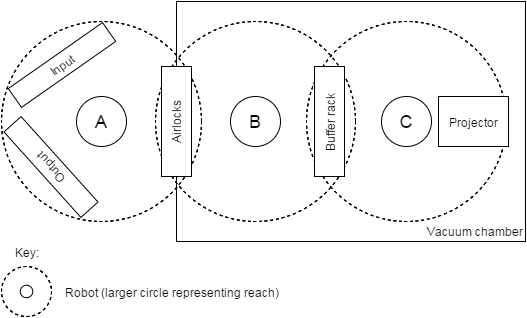
\includegraphics[scale=0.7]{systemmodel}
		\caption{A schematic overview of the system}
		\label{fig:overview}
	\end{figure}
	%TODO[DONE]
	The Extreme Ultraviolet (EUV) Wafer Stepper is a system developed by ASML to treat silicon wafers for the manufacturing of integrated circuits. Treating a wafer means projecting an image onto a silicon wafer with ultra violet light. Since ultra violet radiation is absorbed by air, this treatment has to happen in a vacuum to ensure the accuracy of the projection. This means wafers will have to enter and exit the system through airlocks, also referred to as sluices. The version of the system considered in this document has two sluices. One robot will move wafers from the input to the airlocks or from the airlocks to the output for treated wafers from outside the vacuum chamber. One robot will move wafers from the airlocks to a buffer rack inside the vacuum chamber and vice versa for treated wafers. A last robot, located inside the vacuum chamber, takes wafers from the internal buffer rack to the projector and back once the projector is done. A schematic overview of the system can be found in figure \ref{fig:overview}.\\
	\\
	The goal of this document is to present a model for the controller software of this EUV Wafer Stepper system. This verification ensures that the system behaves according to a predefined list of requirements, which ensure the system does not damage any wafer or system components during operation.
	\section{System components}
	The system can be broken down into individual (physical) components to be considered by the controller software. These components are the following:
	\begin{itemize}
	\item \textbf{Input} - A rack containing untreated wafers located outside of the vacuum chamber.
	\item \textbf{Output} - A rack for treated wafers outside the vacuum chamber.
	\item \textbf{Airlocks} - An array of airlocks providing entrance into the vacuum chamber. Each airlock consists of an inner door, outer door, vacuum pump and air pressure sensor.
	\item \textbf{Buffer Rack} - The buffer rack located inside the vacuum chamber that can temporarily hold wafers.
	\item \textbf{Projector} - The projector inside the vacuum chamber that treats the wafers.
	\item \textbf{Robot A} - The robot that can reach \emph{Input}, \emph{Output} and the \emph{Airlocks}.
	\item \textbf{Robot B} - The robot inside the vacuum chamber that can reach the \emph{Airlocks} and \emph{Buffer Rack}.
	\item \textbf{Robot C} - The other robot inside the vacuum chamber that can reach the \emph{Buffer Rack} and \emph{Projector}.
	\end{itemize}
	
	\chapter{System requirements}
	
	\newcommand{\req}[1]{
		\item[\textbf{R\stepcounter{counter}\arabic{counter}}] {#1}
		\hrule
	}
	
	\newcommand{\reqb}[2]{
		\item[\textbf{{#1}}] {#2}
		\hrule
	}
	
	%TODO[DONE] Add text explaining the purpose of the requirements,
	This chapter contains a list of requirements for the behaviour of the system, which is of course controlled by the controller that is modelled in later chapters. This controller has to ensure these requirements are not violated in the system. Each requirement is a statement about what the system should and should not do. The requirements will be translated in terms of system interactions in chapter 4, making them easier to verify.
	\section{Liveness requirement}
	\begin{itemize}
		\req{Assuming no sluice breaks during operation, every wafer entering the system from the input will unavoidably appear treated on the output.}
	\end{itemize}
	
	\section{Sluice requirements}
	\begin{itemize}
		\req{Only one sluice door can be open at a time.}
		\req{The outer sluice door can only open if there is normal air pressure inside the sluice.}
		\req{The inner sluice door can only open if there is a vacuum inside the sluice.}
		\req{The vacuum pump can only make a vacuum if both sluice doors are closed.}
		\req{The doors of a sluice can not close if a robot is reaching inside.}
	\end{itemize}
	
	\section{Sluice robot requirements}
	\begin{itemize}
		\req{Robot A may only move to a sluice if the outer door of the target sluice is open.}
		\req{Robot B may only move to a sluice if the inside door of the target sluice is open.}
		\req{Robot A\&B may only choose a sluice to put a wafer in that is empty.}
		\req{Robot A\&B may only try to retrieve a wafer from an occupied sluice.}
		\req{Robot A\&B can only put a wafer on an empty spot on the rack.}
		\req{Robot A\&B may only target functioning sluices.}
		\req{Robot A\&B should only try to take wafers from the rack if there are wafers available.}
		\req{Robot B may not access the same spot on the rack as Robot C at the same time.}
	\end{itemize}
	
	\section{Inside robot requirements}
	\begin{itemize}
		\req{Robot C can not access the same spot on the rack as Robot B at the same time.}
		\req{Robot C can not put a wafer on the projection platform when it is occupied.}
		\req{Robot C can not take a wafer from the projection platform if the projection is not done.}
		\req{Robot B\&C can not put a wafer on an occupied place on the rack.}
	\end{itemize}
		
	\section{Projector requirements}
	\begin{itemize}
		\req{The projector only starts its treatment when a wafer is on the projection platform.}
	\end{itemize}
	
	\chapter{System interactions}
	This chapter contains the interactions the controller has with the outside world. The interactions are split up into two sections, Controller-System interactions and System-Controller interactions based on who initiates the interaction. These interaction are the base for the model of the controller software.
\section{Controller-System interactions}
These travel from the controller to the system. The controller-system interactions could be seen as orders to the physical system.
	\begin{itemize}
\item OpenOuterDoor($N$) - Open the outer door of sluice $N$.
\item CloseOuterDoor($N$) - Close the outer door of sluice $N$.
\item OpenInnerDoor($N$) - Open the inner door of sluice $N$.
\item CloseInnerDoor($N$) - Close the inner door of sluice $N$.
\item PumpVacuum($N$) - Start pumping a vacuum in sluice $N$.
\item ReleaseVacuum($N$) - Start releasing the vacuum in sluice $N$.

\item RobotFromInput($W$) - Robot A picks up wafer $W$ from the input rack.
\item RobotToOutput($W$) - Robot A deposits wafer $W$ on the output rack.

\item RobotToSluice($R, S, W$) - Robot $R$ deposits wafer $W$ it is holding in sluice $S$.
\item RobotFromSluice($R, S, W$) - Robot $R$ picks up wafer $W$ from sluice $S$.

\item RobotToRack($R, P, W$) - Robot $R$ deposits wafer $W$ it is holding to position $P$ on the buffer rack.
\item RobotFromRack($R, P, W$) - Robot $R$ takes wafer $W$ from position $P$ on the buffer rack.

\item RobotToProjector($W$) - Robot C deposits wafer $W$ it is holding on the projector.
\item RobotFromProjector($W$) - Robot C picks up wafer $W$ that is currently on the projector.

\item TreatWafer($W$) - The projector treats wafer $W$.
\end{itemize}

	\section{System-Controller interactions}
	These interaction could be seen as events in the physical system. They travel from the system to the controller, for example to let the controller know when some order it gave to the system has been completed.
	\begin{itemize}
\item RobotReset($R$) - Robot $R$ has moved to its default position.
\item OuterDoorOpened($S$) - The outer door of sluice $S$ has completely opened.
\item OuterDoorClosed($S$) - The outer door of sluice $S$ has completely closed.
\item InnerDoorOpened($S$) - The inner door of sluice $S$ has completely opened.
\item InnerDoorClosed($S$) - The inner door of sluice $S$ has completely closed.
\item VacuumDone($S$) - The vacuum in sluice $S$ is complete.
\item VacuumReleased($S$) - The vacuum in sluice $S$ is completely released.
\item WaferTreated($W$) - Wafer $W$ is treated by the projector.
	\end{itemize}
	
	\chapter{Requirements in terms of interactions}
	Since the model of the controller system will consist of sequences of interactions, the requirements from chapter 2 should be translated in terms of these interactions too, to be able to verify them on the model. This chapter contains this translation from textual requirement to a requirement in terms of interactions.
	\section{Liveness requirement}
	\begin{itemize}
		\reqb{SR1}{After RobotFromInput($w$), TreatWafer($w$) should unavoidably happen, followed by RobotToOutput(TreatedWafer($w$)) within finite time.}
	\end{itemize}
	\section{Sluice requirements}
	\begin{itemize}
		\reqb{SR2}{OpenOuterDoor($N$) can only happen after InnerDoorClosed($N$) if no OpenInnerDoor($N$) happened in between.}
		\reqb{SR3}{OpenOuterDoor($N$) can only after VacuumReleased($N$) if no PumpVacuum($N$) happened in between.}
		\reqb{SR4}{OpenInnerDoor($N$) can only happen after PumpVacuum($N$) if no ReleaseVacuum($N$) happened in between(}
		\reqb{SR5}{PumpVacuum($N$) can only happen after InnerDoorClosed($N$) and OuterDoorClosed($N$) if no OpenInnerDoor($N$) or OpenOuterDoor($N$) happened in between.}
		\reqb{SR6}{
\begin{itemize}		
		\item CloseInnerDoor($N$) can only happen after RobotReset($R$) if no  RobotToSluice($R$) or RobotFromSluice($R$) happened in between.
\item closeInnerDoor($N$) can only happen if robotInSluice($N$) is false.
\end{itemize}		
		}
	\end{itemize}
	
	\section{Sluice robot requirements}
	\begin{itemize}
		\reqb{SR7}{RobotToSluice($R_a$,$N$,$w$) or RobotFromSluice($R_a$,$N$,$w$) can only happen after \\
		OuterDoorOpened($N$) if no CloseOuterDoor(N) happened in between.}
		\reqb{SR8}{RobotToSluice($R_b$,$N$,$w$) or RobotFromSluice($R_b$,$N$,$w$) can only happen after \\
		InnerDoorOpened($N$) if no InnerOuterDoor(N) happened in between.}
		\reqb{SR9}{\begin{itemize}
		\item[(a)]  RobotToSluice($R_a$,$N$,$w$) can only happen if \#RobotToSluice($R_a$,$N$,$w$) -\\
		 \#RobotFromSluice($R_b$,$N$,$w$) = 0
		\item[(b)]  RobotToSluice($R_b$,$N$,$w$) can only happen if \#RobotToSluice($R_b$,$N$,$w$) -\\
		 \#RobotFromSluice($R_a$,$N$,$w$) = 0
		\end{itemize}}
		\reqb{SR10}{\begin{itemize}
		\item[(a)]  RobotFromSluice($R_a$,$N$,$w$) can only happen if \#RobotToSluice($R_b$,$N$,$w$) -\\
		 \#RobotFromSluice($R_a$,$N$,$w$) $>$ 0
		\item[(b)]  RobotFromSluice($R_b$,$N$,$w$) can only happen if \#RobotToSluice($R_a$,$N$,$w$) - \\
		\#RobotFromSluice($R_b$,$N$,$w$) $>$ 0
		\end{itemize}}
		\reqb{SR11}{\begin{itemize}
		\item[(a)]  RobotToRack($R_a$,$P$,$w$) can only happen if \#RobotToRack($R_a$,$P$,$w$) - \\
		\#RobotFromRack($R_b$,$P$,$w$) = 0
		\item[(b)]  RobotToRack($R_b$,$P$,$w$) can only happen if \#RobotToRack($R_b$,$P$,$w$) - \\
		\#RobotFromRack($R_a$,$P$,$w$) = 0
		\end{itemize}}
		\reqb{SR12}{RobotToSluice($R$,$N$,$w$) and RobotFromSluice($R$,$N$,$w$) can only happen if SluiceBroken($N$) has not happened.}
		\reqb{SR13}{\begin{itemize}
		\item[(a)]  RobotFromRack($R_a$,$P$,$w$) can only happen if \#RobotToRack($R_a$,$P$,$w$) -\\
		 \#RobotFromRack($R_b$,$P$,$w$) $>$ 0
		\item[(b)]  RobotFromRack($R_b$,$P$,$w$) can only happen if \#RobotToRack($R_b$,$P$,$w$) - \\
		\#RobotFromRack($R_a$,$P$,$w$) $>$ 0
		\end{itemize}}
		\reqb{SR14}{RobotToRack($R_b$,$P$,$w$) can not happen after RobotToRack($R_c$,$P$,$w$) happened without RobotReset($R_c$) in between.}	\end{itemize}
	
	\section{Inside robot requirements}
	\begin{itemize}
		\reqb{SR15}{RobotToRack($R_c$,$P$,$w$) can not happen after RobotToRack($R_c$,$P$,$w$) happened without RobotReset($R_b$) in between.}	
		\reqb{SR16}{RobotToProjector($w$) can if \#RobotToProjector($w$) - \\
		\#RobotFromProjector($w$) = 0.}
		\reqb{SR17}{RobotFromProjector($w$) can not happen if WaferTreated($w$) has not happened.}
		\reqb{SR18}{\begin{itemize}
		\item[(a)] RobotToRack($R_b$,$P$,$w$) can only happen if \#RobotToRack($R_b$,$P$,$w$) - \\
		\#RobotFromRack($R_b$,$P$,$w$) + \#RobotToRack($R_c$,$P$,$w$) - \\
		\#RobotFromRack($R_c$,$P$,$w$) = 0
		\item[(b)] RobotToRack($R_c$,$P$,$w$) can only happen if \#RobotToRack($R_b$,$P$,$w$) - \\
		\#RobotFromRack($R_b$,$P$,$w$) + \#RobotToRack($R_c$,$P$,$w$) - \\
		\#RobotFromRack($R_c$,$P$,$w$) = 0
		 \end{itemize}}
	\end{itemize}
	\section{Projector requirements}
	\begin{itemize}
		\reqb{SR19}{
				TreatWafer($w$) can only happen if WaferToProject($w$) happened with no WaferFromProjector($w$) in between.
		}
	\end{itemize}
	
	\chapter{System model}
	\section{Model overview}
	%TODO review (maybe expand a little bit).
	\begin{figure}
		\centering
		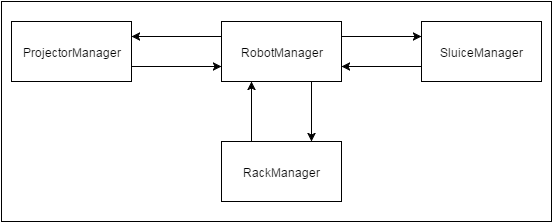
\includegraphics[scale=0.7]{schematicoverview}
		\caption{A schematic overview of the software components}
		\label{fig:components}
	\end{figure}
	To verify the system, a model of the software is made. The software is split up into the following three components:
	\begin{itemize}
	\item \textbf{SluiceManager} - This component manages the sluices, it runs parallel for each sluice. The purpose of this component is to control the individual airlocks.
	\item \textbf{RobotManager} - This component manages the different robots in the system, and runs a parallel process for each robot.
	\item \textbf{ProjectorManager} - The projector is managed by this component.
	\item \textbf{RackManager} - This component's purpose is to monitor the rack.
	\end{itemize}
	
	A schematic view of this system can also be found in figure \ref{fig:components}.
	
	\section{Formal model}
	First the different sorts present in the model are defined.\\
	%Sorts
	\textbf{sort}\\
	\phantom{----} Wafer = \textbf{struct} \emph{wafer}$( id:\mathbb{Z}, treated:\mathbb{B} ) | Dummy?IsDummy$;\\
	\phantom{----} WaferSet = Set( Wafer );\\
	\phantom{----} WaferList = List( Wafer );\\
	\phantom{----} RobotID = \textbf{struct} $R_a | R_b | R_c$;\\
	\phantom{----} SluiceID = \textbf{struct} $S_0 | S_1$;\\
	\phantom{----} SluiceDoorState = \textbf{struct} $inner\_open|closed|outer\_open$;\\
	\\
	Some global parameters can be defined that hold for the system.\\
	%Params
	\textbf{eqn}\\
	\phantom{----} RackSize = 2;\\
	%TODO Explain X
	\phantom{----} NumWafers = $X$;\\
	\phantom{----} NumSluices = 2;\\
	\\
	Some helper-equations are defined. The names are self-explanatory.\\
	%Helper equations
	\textbf{eqn}\\
	\phantom{----} OnRack$( p ) = 0 \leq p < \text{RackSize}$;\hfill for all $p \in \mathbb{N}$\\
	\phantom{----} TreatedWafer(  \emph{wafer}$( w, b )$ ) =  \emph{wafer}$( w, true )$;\hfill for all $w \in \mathbb{Z}, b \in \mathbb{B}$\\
	\\
	\phantom{----} \emph{For all $l \in \text{WaferList}, p \in \mathbb{N}, w \in \text{Wafer}$, where OnRack($p$) = true}:\\
	\phantom{----} PutInList$( [], p, w )$ = [];\\
	\phantom{----} PutInList$( l, p, w )$ = $w$ $|>$ PutInList$( tail( l ), p, w )$;\hfill if $0 < \#l \land \#l = \text{RackSize} - p$\\
	\phantom{----} PutInList$( l, p, w )$ = $ head( l )$ $|>$ PutInList$( tail( l ), p, w )$;\hfill if $0 < \#l \land \#l \neq \text{RackSize} - p$\\
	\\
	\phantom{----} InitRack( 0 ) = [];\\
	\phantom{----} InitRack( n ) = $Dummy |> InitRack( n - 1 )$;\hfill for all $n \in \mathbb{N}$\\
	\\
	\phantom{----} InitWaferList( 0 ) = [];\\
	\phantom{----} InitWaferList( n ) = \emph{wafer}($n$, \emph{false}) $|>$ InitWaferList( n - 1 );\hfill for all $n \in \mathbb{N}$\\
	\\
	The main part of the system model are the processes that make up the system. There is one process for each of the four components in the system. Multiple instances of each process can be run in parallel with different parameters, as explained at the initialisation.\\
	\\%Processes
	The first process is the robot process, consisting of three parts, one for each robot. Each model waits for its RobotReset event after each action before continuing. This event might require a synchronisation step if two components are waiting for the same event.\\
	If robot A is holding a treated wafer it will put it down on the output. If it is holding an untreated wafer, it will try to put it in a sluice and increase its counter. If robot A is not holding anything, it will either take a wafer from one of the sluices if there is one available and decrease its counter, or if the input list is not empty, and the robot's counter is less than the number of sluices, it will pick up a new wafer from the input. The purpose of the counter is to prevent the robot from picking up a wafer when there are no sluices available to put it down in.\\
	If robot B is holding a treated wafer it will try to put it in one of the sluices. If it is holding an untreated wafer, it will put it down on the rack. If robot B is not holding a wafer, it will try to take an untreated wafer from the sluices, or take a treated wafer from the rack.\\
	Robot C will put a wafer on the projector if it is holding an untreated wafer. It will then wait until the projector is done before picking up the wafer again and putting it back on the rack. If robot C is not holding anything and is not waiting for the projector it will try to pick up a wafer from the rack.\\
	{\small
	%Robot
	\textbf{proc}\\
	\phantom{---} R( \emph{rID}:RobotID, $occupied$:$\mathbb{B}$, $w$:Wafer, $in$:WaferList, $out$:WaferSet, $c$:$\mathbb{N}$ ) =\\
	\phantom{-------} \emph{rID} = $R_a \rightarrow$\\
	\phantom{----------} $occupied$ $\rightarrow$\\
	\phantom{--------------} treated($w$)$\rightarrow$RobotToOutput($w$)$\cdot$RobotReset(\emph{rID})$\cdot$R(\emph{rID},$false$,Dummy,$in$,$out$+$\{w\}$,$c$)\\
	\phantom{--------------} $\Diamond \sum\nolimits_{s \in \text{SluiceID}}\cdot$R2S\_R(\emph{rID},$s$,$w$)$\cdot$RReset\_O(\emph{rID})$\cdot$R(\emph{rID},$false$, Dummy,$in$,$out$,$c$+$1$)\\
	\phantom{----------} $\Diamond$\\
	\phantom{--------------} $in \neq [] \land c < NumSluices \rightarrow$ ( RobotFromInput( head($in$) )$\cdot$\\
	\phantom{---------------------} RobotReset(\emph{rID}))$\cdot$R(\emph{rID},$true$,head($in$),tail($in$),$out$,$c$) ) \\
	\phantom{--------------} + $\sum\nolimits_{w_2 \in \text{Wafer}, s \in \text{SluiceID}}$S2R\_R(\emph{rID},$s$,$w_2$)$\cdot$RReset\_D(\emph{rID})$\cdot$R(\emph{rID}, $true$,$w_2$,$in$,$out$,$c$-$1$)\\
	\\
	\phantom{-------} + \emph{rID} = $R_b \rightarrow$\\
	\phantom{----------} $occupied$ $\rightarrow$\\
	\phantom{--------------} treated($w$)$\rightarrow\sum\nolimits_{s\in\text{SluiceID}}$R2S\_R(\emph{rID},$s$,$w$)$\cdot$RReset\_O(\emph{rID})$\cdot$R(\emph{rID},\emph{false},Dummy,$in$,$out$,$c$)\\
	\phantom{--------------} $\Diamond \sum\nolimits_{p\in \mathbb{N}}$OnRack($p$)$\rightarrow$R2Rack\_R(\emph{rID},$p$,$w$)$\cdot$RReset\_O(\emph{rID})$\cdot$R(\emph{rID},\emph{false},Dummy,$in$,$out$,$c$)
	\phantom{----------}  $\Diamond$\\
	\phantom{--------------} $\sum\nolimits_{w_2 \in \text{Wafer}, s \in \text{SluiceID}}$S2R\_R(\emph{rID},$s$,$w_2$)$\cdot$RReset\_D(\emph{rID})$\cdot$R(rID,\emph{true},$w_2$,$in$,$out$,$c$)\\
	\phantom{--------------} +$\sum\nolimits_{w_2 \in \text{Wafer}, p \in \mathbb{N}}$treated($w_2$)$\land$OnRack($p$)$\rightarrow$Rack2R\_R(\emph{rID},$p$,$w_2$)$\cdot$\\
	\phantom{-----------------------------} RReset(\emph{rID})$\cdot$R(\emph{rID},\emph{true},$w_2$,$in$,$out$,$c$)\\
	\\
	\phantom{-------} + \emph{rID} = $R_c \rightarrow$\\
	\phantom{----------} $occupied$ $\rightarrow$\\
	\phantom{--------------} R2P\_R($w$)$\cdot$RReset\_O(\emph{rID})$\cdot$P2R\_R(TreatedWafer($w$))$\cdot$RReset\_D(\emph{rID})$\cdot\sum\nolimits_{p \in \mathbb{N}}$OnRack($p$)$\rightarrow$\\
	\phantom{------------------} R2Rack\_R(\emph{rID},$p$,TreatedWafer($w$))$\cdot$RReset\_O(\emph{rID})$\cdot$R(\emph{rID},\emph{false},Dummy,$in$,$out$,$c$)\\
	\phantom{----------} $\Diamond$\\
	\phantom{--------------} +$\sum\nolimits_{w_2 \in \text{Wafer}, p \in \mathbb{N}}\neg$treated($w_2$)$\land$OnRack($p$)$\rightarrow$Rack2R\_R(\emph{rID},$p$,$w_2$)$\cdot$\\
	\phantom{-----------------------------} RReset\_D(\emph{rID})$\cdot$R(\emph{rID},\emph{true},$w_2$,$in$,$out$,$c$);
	}\\
	\\
	The sluice process holds parameters for its id, if it is occupied or not, the wafer that is in that wafer, the state of the door and if the sluice is broken or not. Sluices will wait until robots have returned to their rest position before closing their doors. If there is no wafer in the sluice and the inner/outer door is open, the sluice will accept a wafer from robot B/robot A respectively and start closing. If there is a wafer in the sluice and the inner/outer door is open, the sluice will wait until robot B/robot A respectively takes the wafer out of it. If the doors of a sluice are closed and the wafer inside is treated, the sluice will release the vacuum. Once the vacuum is released it will start opening the outer doors. If the sluice doors are closed and there is an untreated wafer inside, the sluice will pumping a vacuum. If the vacuum is done the sluice will open its inner doors. On top of this the sluice could non-deterministically break at any point.\\
	Note: This protocol for the sluices means that there can never be more wafers in the vacuum chamber than the number of sluices. Therefore the spaces on the rack could be limited to the number of sluices in the system.\\
	%Sluice
	{\small
	\textbf{proc}\\
	\phantom{---} S( $id$:SluiceID, $occupied$:$\mathbb{B}$, $w$:Wafer, $door$:DoorState, $broken$:$\mathbb{B}$ ) =\\
	\phantom{------} $\neg broken \rightarrow$\\
	\phantom{---------} $\neg occupied \rightarrow$\\
	\phantom{-------------} $door=outer\_open \rightarrow\sum\nolimits_{w_2\in \text{Wafer}}$R2S\_S($R_a$,$id$,$w_2$)$\cdot$RReset\_D($R_a$)$\cdot$CloseOuterDoor($id$)$\cdot$\\
	\phantom{-----------------} OuterDoorClosed($id$)$\cdot$PumpVacuum($id$)$\cdot$VacuumDone($id$)$\cdot$S($id$,\emph{true},$w_2$,$closed$,\emph{false})\\
	\phantom{-------------} + $door=inner\_open \rightarrow\sum\nolimits_{w_2\in \text{Wafer}}$R2S\_S($R_b$,$id$,$w_2$)$\cdot$RReset\_D($R_b$)$\cdot$CloseInnerDoor($id$)$\cdot$\\
	\phantom{-----------------} InnerDoorClosed($id$)$\cdot$ReleaseVacuum($id$)$\cdot$VacuumReleased($id$)$\cdot$S($id$,\emph{true},$w_2$,$closed$,\emph{false})\\
	\phantom{---------} $\Diamond$\\
	\phantom{-------------} $door=outer\_open \rightarrow$S2R\_S($R_a$,$id$,$w$)$\cdot$RReset\_O($R_a$)$\cdot$S($id$,\emph{false},Dummy,$door$,\emph{false})\\
	\phantom{-------------} + $door=inner\_open \rightarrow$S2R\_S($R_b$,$id$,$w$)$\cdot$RReset\_O($R_b$)$\cdot$S($id$,\emph{false},Dummy,$door$,\emph{false})\\
	\phantom{---------} + $door=closed \land \text{IsTreated}(w) \rightarrow$\\
	\phantom{-------------} OpenOuterDoor($id$) $\cdot$ OuterDoorOpened($id$) $\cdot$ S($id$, $occupied$, $w$, $outer\_open$, \emph{false})\\
	\phantom{---------} + $door=closed \land \neg\text{IsTreated}(w) \rightarrow$\\
	\phantom{-------------} OpenInnerDoor($id$) $\cdot$ InnerDoorOpened($id$) $\cdot$ S($id$, $occupied$, $w$, $inner\_open$, \emph{false})\\
	\phantom{---------} + SluiceBroken($id$) $\cdot$ S($id$, $occupied$, $w$, $door$, \emph{true});\\
	}\\
	The projector process keeps track of if there is a wafer inside, and which wafer that is. If the projector is occupied, it will treat the wafer and once that is done wait until the wafer was picked up by robot C before going back to its unoccupied state. If there is no wafer on the projector it will accept a wafer from robot C.\\
	%Projector
	{\small
	\textbf{proc}\\
	\phantom{---} P( $occupied$:$\mathbb{B}$, $w$:Wafer ) =\\
	\phantom{------} $occupied\rightarrow$\\
	\phantom{---------} TreatWafer($w$)$\cdot$WaferTreated($w$)$\cdot$P2R\_P(TreatedWafer($w$))$\cdot$RReset\_O($R_c$)$\cdot$P(\emph{false},Dummy)\\
	\phantom{------} $\Diamond$\\
	\phantom{---------} $\sum\nolimits_{w_2\in \text{Wafer}}$ R2P\_P($w_2$) $\cdot$ RReset\_D($R_c$) $\cdot$ P(\emph{true}, $w_2$);
	}\\
	The rack process is just to \\
	%Rack
	{\small
	\textbf{proc}\\
	\phantom{---} Rack( $wl$:WaferList ) =\\
	\phantom{-------} $\sum\nolimits_{w\in \text{Wafer}, p \in \mathbb{N}, r \in \text{RobotID}}$ OnRack($p$) $\rightarrow$ IsDummy( $wl.p$ ) $\rightarrow$\\
	\phantom{-----------} R2Rack\_Rack($r$, $p$, $w$) $\cdot$ RReset\_D($r$) $\cdot$ Rack(PutInList($wl$, $p$, $w$))\\
	\phantom{-------} + $\sum\nolimits_{p \in \mathbb{N}, r \in \text{RobotID}}$ OnRack( $p$ ) $\rightarrow \neg$IsDummy($wl.p$)$\rightarrow$\\
	\phantom{-----------} Rack2R\_Rack($r$, $p$, $wl.p$) $\cdot$ RReset\_O( $r$ ) $\cdot$ Rack(PutInList($wl$, $p$, Dummy));
	}\\

	The initialisation of the system without any hiding and all steps allowed can be found below. Note the RobotReset synchronisation of steps RReset\_O(rigin) and RReset\_D(estination), which is for when two components are waiting on the same RobotReset event. An instance of the robot process is started for each process. Robot A recievs the input list, since robot A is the only robot that can reach the input. This is the entry point for wafers into the system.\\
	A process is initialised for the rack with a list of dummies equal to the size of the rack.\\
	For each sluice a parallel instance of the sluice process is started. Each sluice is empty initially and has the outer doors open.\\
	A process is started for the projector that is empty at the start.\\
	%Initialisation\\
	\textbf{init}\\
	$\nabla_{\text{ \{RobotToSluice, RobotFromSluice, RobotToProjector, RobotFromProjector, RobotToRack, RobotFromRack,}}$\\
	\phantom{--} $_{ \text{ RobotFromInput, RobotFromOutput,}}$\\
	\phantom{--} $_{ \text{ CloseOuterDoor, CloseInnerDoor, OpenInnerDoor, OpenOuterDoor, PumpVacuum, ReleaseVacuum,}}$\\
	\phantom{--} $_{ \text{ RobotReset, WaferTreated, OuterDoorOpened, OuterDoorClosed, InnerDoorOpened, InnerDoorClosed, VacuumDone, VacuumReleased,}}$\\
	\phantom{--} $_{ \text{SluiceBroken\}}}$(\\
	\phantom{---} $\Gamma_{\{R2S\_R|R2S\_S\rightarrow RobotToSluice,S2R\_S|S2R\_R\rightarrow RobotFromSluice,}$\\
	\phantom{-----} $_{ R2P\_R|R2P\_P\rightarrow RobotToProjector, P2R\_P|P2R\_R\rightarrow RobotFromProjector,}$\\
	\phantom{-----} $_{ R2Rack\_R|R2Rack\_P\rightarrow RobotToRack, Rack2R\_P|Rack2R\_R\rightarrow RobotFromRack,}$\\
	\phantom{-----} $_{ RReset\_O|RReset\_D\rightarrow RobotReset \}}$(\\
	\phantom{---------} R( $R_a$, \emph{false}, $Dummy$, \emph{InitWaferList(NumWafers)}, $\emptyset$, 0 ) $||$\\
	\phantom{---------} R( $R_b$, \emph{false}, $Dummy$, [], $\emptyset$, 0 ) $||$\\
	\phantom{---------} R( $R_c$, \emph{false}, $Dummy$, [], $\emptyset$, 0 ) $||$\\
	\phantom{---------} Rack( $InitRack(RackSize)$ ) $||$\\
	\phantom{---------} S( $S_0$, \emph{false}, $Dummy$, $outer\_open$, \emph{false} ) $||$\\
	\phantom{---------} S( $S_1$, \emph{false}, $Dummy$, $outer\_open$, \emph{false} ) $||$\\
	\phantom{---------} P( \emph{false}, $Dummy$ )\\
	\phantom{---} )\\
	);
	
	\chapter{Verification}

    \section{Requirement verification}

    \textbf{Traceability matrix}\\
    \begin{tabular}{| l | l | l | }
        \hline
        Requirement ID & System Requirement ID & Modal formula ID \\ \hline
        R1 & SR1 & MCF1 \\ \hline
        R2 & SR2 & MCF2inner, MCF2outer \\ \hline
        R3 & SR3 & MCF3 \\ \hline
        R4 & SR4 & MCF4 \\ \hline
        R5 & SR5 & MCF5 \\ \hline
        R6 & SR6 & MCF6a1, MCF6a2, MCF6b1, MCF6b2 \\ \hline
        R7 & SR7 & MCF71, MCF72 \\ \hline
        R8 & SR8 & MCF82, MCF82 \\ \hline
        R9 & SR9 & MCF9a, MCF9b \\ \hline
        R10 & SR10 & MCF10a, MCF10b \\ \hline
        R11 & SR11 & MCF11 \\ \hline
        R12 & SR12 & MCF12 \\ \hline
        R13 & SR13 & MCF13rb, MCF13rc \\ \hline
        R14 & SR14 & MCF14 \\ \hline
        R15 & SR15 & MCF15 \\ \hline
        R16 & SR16 & MCF16 \\ \hline
        R17 & SR17 & MCF17 \\ \hline
        R18 & SR18 & MCF18 \\ \hline
        R19 & SR19 & MCF19 \\  \hline
    \end{tabular}

    \pagebreak

    %TODO make this a section instead, add a little explanation.
    %TODO Fix the weird outlining (caused by longtable?) [done]
    %TODO Fix requirements. 13,18,19 need to be looked at still

    \textbf{Modal $\mu$-calculus formulas}\\

    \textbf{MCF1}
    \begin{multline*}
        [true^{\star}] \forall w \in Wafer. [WaferFromInput(w)]\\
        \mu X.([RobotToOutput(TreatedWafer(w))]X \wedge \langle true \rangle true)
    \end{multline*}

    \textbf{MCF2inner}
    \begin{multline*}
        \forall s \in SluiceID.[true^{\star}.InnerDoorOpened(s).\overline{InnerDoorClosed(s)}^{\star}\\
        .OpenOuterDoor(s)]false
    \end{multline*}

    \textbf{MCF2outer}
    \begin{multline*}
        \forall s \in SluiceID.[true^{\star}.OuterDoorOpened(s).\overline{OuterDoorClosed(s)}^{\star}\\
        .OpenInnerDoor(s)]false
    \end{multline*}

    \textbf{MCF3}
    \begin{multline*}
        [true^{\star}] \forall s \in SluiceID. [PumpVacuum(s).\overline{ReleaseVacuum}^{\star}.OpenOuterDoor(s)]true
    \end{multline*}

    \textbf{MCF4}
    \begin{multline*}
        \forall s \in SluiceID.[true^{\star}.ReleaseVacuum(s).\overline{PumpVacuum}^{\star}.OpenInnerDoor(s)]true
    \end{multline*}

    \textbf{MCF5}
    \begin{multline*}
        \forall s \in SluiceID.[true^{\star}.(OpenInnerDoor(s).\overline{InnerDoorClose(s)}^{\star}.PumpVacuum(s)\\
        \vee OpenOuterDoor(s).\overline{OpenOuterDoorClose(s)}^{\star}.PumpVacuum(s))]false
    \end{multline*}

    \textbf{MCF6a1}
    \begin{multline*}
        [true^{\star}] \forall w \in Wafer, s \in SluiceID.[RobotFromSluice(Ra,s,w).\overline{RobotReset(Ra)}^{\star}\\
        .CloseOuterDoor(s)]false
    \end{multline*}

    \textbf{MCF6a2}
    \begin{multline*}
        [true^{\star}] \forall w \in Wafer, s \in SluiceID.[RobotToSluice(Ra,s,w).\overline{RobotReset(Ra)}^{\star} \\
        .CloseOuterDoor(s)]false
    \end{multline*}
	
    \textbf{MCF6b1}
    \begin{multline*}
        [true^{\star}] \forall w \in Wafer, s \in SluiceID.[RobotFromSluice(Rb,s,w).\overline{RobotReset(Rb)}^{\star}\\
        .CloseInnerDoor(s)]false
    \end{multline*}

    \textbf{MCF6b2}
    \begin{multline*}
        [true^{\star}] \forall w \in Wafer, s \in SluiceID.[RobotToSluice(Rb,s,w).\overline{RobotReset(Rb)}^{\star} \\
        .CloseInnerDoor(s)]false
    \end{multline*}

    \textbf{MCF71}
    \begin{multline*}
        [true^{\star}] \forall w \in Wafer, s \in SluiceID.[OuterDoorClosed(s).\overline{OuterDoorOpened}^{\star} \\
        .RobotToSluice(Ra,s,w)]false
    \end{multline*}

    \textbf{MCF72}
    \begin{multline*}
        [true^{\star}] \forall w \in Wafer, s \in SluiceID.[OuterDoorClosed(s).\overline{OuterDoorOpened}^{\star} \\
        .RobotFromSluice(Ra,s,w)]false
    \end{multline*}

    \textbf{MCF81}
    \begin{multline*}
        [true^{\star}] \forall w \in Wafer, s \in SluiceID.[InnerDoorClosed(s).\overline{InnerDoorOpened(s)}^{\star} \\
        .RobotToSluice(Rb, s, w)]false
    \end{multline*}

    \textbf{MCF82}
    \begin{multline*}
        [true^{\star}] \forall w \in Wafer, s \in SluiceID.[InnerDoorClosed(s).\overline{InnerDoorOpened(s)}^{\star} \\
        .RobotFromSluice(Rb, s, w)]false
    \end{multline*}

    \textbf{MCF9a}
    \begin{multline*}
        [true^{\star}] \forall w1,w2 \in Wafer, s in SluiceID.[RobotToSluice(Ra,s,w1) \\
        .\overline{RobotFromSluice(Rb,s,w1)}^{\star}. \exists w2 \in Wafer. RobotToSluice(Ra,s,w2)]false
    \end{multline*}

    \textbf{MCF9b}
    \begin{multline*}
        [true^{\star}] \forall w1 \in Wafer, s \in SluiceID.[RobotToSluice(Rb,s,w1)\\
        .\overline{RobotFromSluice(Ra,s,w1)}^{\star}. \exists w2 \in Wafer. RobotToSluice(Rb,s,w2)]false
    \end{multline*}

    \textbf{MCF10a}
    \begin{multline*}
        \nu X(i=0). \forall s \in SluiceID. [\forall w1 \in Wafer. \overline{RobotToSluice(Rb,s,w1)} \\
        \wedge \forall w2 \in Wafer. \overline{RobotFromSluice(Ra,s,w2)}] X(i) \\
        \wedge [\exists w3 \in Wafer. RobotToSluice(Rb,s,w3)]X(i+1) \\
        \wedge [\exists w4 \in Wafer.RobotFromSluice(Ra,s,w4)](i>0 \wedge X(i-1))
    \end{multline*}

    \textbf{MCF10b}
    \begin{multline*}
        \nu X(i=0). \forall s \in SluiceID. [\forall w1 \in Wafer. \overline{RobotToSluice(Ra,s,w1)} \\
        \wedge \forall w2 \in Wafer. \overline{RobotFromSluice(Rb,s,w2)}] X(i) \\
        \wedge [\exists w3 \in Wafer. RobotToSluice(Ra,s,w3)]X(i+1) \\
        \wedge [\exists w4 \in Wafer.RobotFromSluice(Rb,s,w4)](i>0 \wedge X(i-1))
    \end{multline*}

    \textbf{MCF11}
    \begin{multline*}
        [true^{\star}] \forall p \in \mathbb{N}, r \in RobotID, w \in Wafer. [RobotToRack(r,p,w)\\
        .\overline{RobotFromRack(r,p,w)}^\star.RobotToRack(r,p,w)]false
    \end{multline*}

    \textbf{MCF12}
    \begin{multline*}
        [true^{\star}] \forall s \in SluiceID [SluiceBroken(s).true^{\star}.(CloseInnerDoor(s) \\
        \vee CloseOuterDoor(s) \vee OpenInnerDoor(s) \\
        \vee OpenOuterDoor(s) \vee PumpVacuum(s) \\
        \vee ReleaseVacuum(s) \vee SluiceBroken(s))]false
    \end{multline*}

    \textbf{MCF13rb}
    \begin{multline*}
        [true^{\star}] \forall p \in \mathbb{N}, w \in Wafer.[\overline{RobotToRack(Rb,p,w}^{\star}.RobotFromRack(Rc, p, w)]false
    \end{multline*}

    \textbf{MCF13rc}
    \begin{multline*}
        [true^{\star}] \forall p \in \mathbb{N}, w \in Wafer.[\overline{RobotToRack(Rc,p,w}^{\star}.RobotFromRack(Rb, p, w)]false
    \end{multline*}

    \textbf{MCF14}
    \begin{multline*}
        [true^{\star}] \forall p \in \mathbb{N}, w \in Wafer. [(RobotToRack(Rc,p,w) \vee RobotFromRack(Rc,p,w))\\
        .\overline{RobotReset(Rc}^{\star}.(RobotRack(Rb,p,w) \vee RobotFromRack(Rb,p,w)]false
    \end{multline*}

    \textbf{MCF15}
    \begin{multline*}
        [true^{\star}] \forall p \in \mathbb{N}, w \in Wafer. [(RobotToRack(Rb,p,w) \vee RobotFromRack(Rb,p,w))\\
        .\overline{RobotReset(Rb}^{\star}.(RobotRack(Rc,p,w) \vee RobotFromRack(Rc,p,w)]false
    \end{multline*}

    \textbf{MCF16}
    \begin{multline*}
        [true^{\star}] \forall w,w2 \in Wafer. [RobotToProjector(w).\overline{RobotFromProjector(w)}^{\star} \\
        .RobotToProjector(w2)]false
    \end{multline*}

    \textbf{MCF17}
    \begin{multline*}
        [true^{\star}] \forall w \in Wafer. [RobotToProjector(w).\overline{TreatWafer(W)}^{\star}\\
        .RobotFromProjector(w)]false \\
    \end{multline*}

    \textbf{MCF18}
    \begin{multline*}
        [true^{\star}] \forall w \in Wafer, p \in \mathbb{N}. [RobotToRack(Rc, p, w).\overline{RobotFromRack(Rb,p,w)}^{\star} \\
        .RobotToRack(Rc,p,w)]false
    \end{multline*}

    \textbf{MCF19}
    \begin{multline*}
        [true^{\star}] \forall w \in Wafer. [RobotToProjector(w).true^{\star}.RobotFromProjector(w).true^{\star} \\
        .TreatWafer(w)]false
    \end{multline*}

	\section{Verification procedure}
	%TODO[DONE] Add Commands used, System specifications the tests were run on (OS etc)
	Several steps were taken to verify the correctness of this model. First, the model was translated into mCRL2 syntax. Next, all modal formulas were translated into the mcf format used by the mCRL2 tools. Once both translations were done, a linear process specification was generated from the mCRL2 input (using mcrl22lps). This LPS was used to verify the requirements by generating a parameterized boolean expression system for each modal formula (using the lps2pbes tool) and evaluating this expression by running pbes2bool.\\
	For the verification of the system release version 201409.1.13218 of the mCRL2 tools was used. Furthermore, verification process was performed on windows 7 as well as windows 8. \\
	\\
	The system was verified for wafer counts from 1 to 5 to avoid any statespace problems. This should nonetheless present an accurate view of the system, as the maximum amount of wafers inside the vacuum chamber is at most the number of sluices, which is two.
	
	\section{Verification results}
	Results of the verification: All modal formulas evaluated to true. Thus all requirements are met by the system.
	
	%TODO Add mcrl2 code appendix
	%TODO Add plain-text modal formulas Appendix
	\section{Appendix A}
	\textbf{Modal $\mu$-calculus formulas in plain text}\\

    \textbf{MCF1}
    \begin{lstlisting}
    	[true*] forall w: Wafer. [RobotFromInput(w)] mu X. ([!RobotToOutput(TreatedWafer(w))]X && <true>true)
    \end{lstlisting}

    \textbf{MCF2a}
    \begin{lstlisting}
       forall s: SluiceID . [true* . InnerDoorOpened(s) . (!InnerDoorClosed(s))* . OpenOuterDoor(s)] false
       \end{lstlisting}

    \textbf{MCF2b}
    \begin{lstlisting}
       forall s: SluiceID . [true* . OuterDoorOpened(s) . (!OuterDoorClosed(s))* . OpenInnerDoor(s)] false
       \end{lstlisting}

    \textbf{MCF3}
    \begin{lstlisting}
       [true*] forall s: SluiceID . [ PumpVacuum(s) . (!ReleaseVacuum(s))* .  OpenOuterDoor(s)] true
       \end{lstlisting}

    \textbf{MCF4}
    \begin{lstlisting}
        forall s: SluiceID . [true* . ReleaseVacuum(s) . (!PumpVacuum(s))* .  OpenInnerDoor(s)] true
        \end{lstlisting}

    \textbf{MCF5}
    \begin{lstlisting}
       forall s: SluiceID . [true* . (OpenInnerDoor(s). (!InnerDoorClosed(s))* . PumpVacuum(s)  + OpenOuterDoor(s). (!OuterDoorClosed(s))* . PumpVacuum(s))] false
       \end{lstlisting}

    \textbf{MCF6a1}
    \begin{lstlisting}
       [true*] forall w:Wafer, s:SluiceID . [RobotFromSluice(Ra,s,w) . (!RobotReset(Ra))* . CloseOuterDoor(s)] false
       \end{lstlisting}

    \textbf{MCF6a2}
    \begin{lstlisting}
       [true*] forall w:Wafer, s:SluiceID . [RobotToSluice(Ra,s,w) . (!RobotReset(Ra))* . CloseOuterDoor(s)] false
    \end{lstlisting}
	
    \textbf{MCF6b1}
    \begin{lstlisting}
      [true*] forall w:Wafer, s:SluiceID . [RobotFromSluice(Rb,s,w) . (!RobotReset(Rb))* . CloseInnerDoor(s)] false
    \end{lstlisting}

    \textbf{MCF6b2}
    \begin{lstlisting}
        [true*] forall w:Wafer, s:SluiceID . [RobotToSluice(Rb,s,w) . (!RobotReset(Rb))* . CloseInnerDoor(s)] false
    \end{lstlisting}

    \textbf{MCF7a}
    \begin{lstlisting}
       [true*] forall  s:SluiceID . [OuterDoorClosed(s) . (!OuterDoorOpened(s))* ] forall w:Wafer . [RobotToSluice(Ra, s, w)] false
    \end{lstlisting}

    \textbf{MCF7b}
    \begin{lstlisting}
       [true*] forall  s:SluiceID . [OuterDoorClosed(s) . (!OuterDoorOpened(s))* ] forall w:Wafer . [RobotFromSluice(Ra, s, w)] false
    \end{lstlisting}

    \textbf{MCF8a}
    \begin{lstlisting}
        [true*] forall  s:SluiceID . [InnerDoorClosed(s) . (!InnerDoorOpened(s))* ] forall w:Wafer . [RobotToSluice(Rb, s, w)] false
    \end{lstlisting}

    \textbf{MCF8b}
    \begin{lstlisting}
     [true*] forall  s:SluiceID . [InnerDoorClosed(s) . (!InnerDoorOpened(s))* ] forall w:Wafer . [RobotFromSluice(Rb, s, w)] false
    \end{lstlisting}

    \textbf{MCF9a}
    \begin{lstlisting}
       [true*] forall w1:Wafer, s:SluiceID . [RobotToSluice(Ra,s,w1) . (!RobotFromSluice(Rb,s,w1))* . exists w2: Wafer . RobotToSluice(Ra,s,w2)] false
    \end{lstlisting}

    \textbf{MCF9b}
    \begin{lstlisting}
       [true*] forall w1:Wafer, s:SluiceID . [RobotToSluice(Rb,s,w1) . (!RobotFromSluice(Ra,s,w1))* . exists w2: Wafer . RobotToSluice(Rb,s,w2)] false
    \end{lstlisting}

    \textbf{MCF10a}
    \begin{lstlisting}
       nu X( i:Int=0 ). forall w1,w2:Wafer. forall s:SluiceID. [!RobotToSluice(Rb,s,w1) && !RobotFromSluice(Ra,s,w2)]X(i) && exists w3: Wafer. [RobotToSluice(Rb,s,w3)]X(i+1) && exists w4: Wafer .[RobotFromSluice(Ra,s,w4)](val(i > 0) && X(i-1)) 
    \end{lstlisting}

    \textbf{MCF10b}
    \begin{lstlisting}
nu X( i:Int=0 ). forall w1,w2:Wafer. forall s:SluiceID. [!RobotToSluice(Ra,s,w1) && !RobotFromSluice(Rb,s,w2)] X(i) && exists w3: Wafer . [ RobotToSluice(Ra,s,w3)]X(i+1) && exists w4: Wafer .[RobotFromSluice(Rb,s,w4)](val(i > 0) && X(i-1))
    \end{lstlisting}

    \textbf{MCF11}
    \begin{lstlisting}
       [true*] forall p:Nat, r:RobotID, w:Wafer. [RobotToRack(r,p,w).(!RobotFromRack( r,p,w)) .RobotToRack(r,p,w)]false
    \end{lstlisting}

    \textbf{MCF12}
    \begin{lstlisting}
       [true*] forall s:SluiceID. [SluiceBroken(s).true*.(CloseInnerDoor(s) + CloseOuterDoor(s) + OpenInnerDoor(s) + OpenOuterDoor(s) + PumpVacuum(s) + ReleaseVacuum(s) + SluiceBroken(s))]false
    \end{lstlisting}

    \textbf{MCF13a}
    \begin{lstlisting}
     nu X( i:Int=0 ). forall w1,w2:Wafer. forall p:Nat. val(p<=RackSize)=> [!RobotToRack(Rb,p,w1) && !RobotFromRack(Rc,p,w2)] X(i) 
&& exists w3:Wafer . [RobotToRack(Rb,p,w3)]X(i+1) && exists w4:Wafer . [RobotFromRack(Rc,p,w4)](val(i > 0) && X(i-1))
    \end{lstlisting}

    \textbf{MCF13b}
    \begin{lstlisting}
       nu X( i:Int=0 ). forall w1,w2,w3,w4:Wafer. forall p:Nat. val(p<=RackSize)=> [!RobotToRack(Rc,p,w1) && !RobotFromRack(Rb,p,w2)] X(i) 
&& [RobotToRack(Rc,p,w3)]X(i+1) && [RobotFromRack(Rb,p,w4)] (val(i > 0) && X(i-1))
   \end{lstlisting}

    \textbf{MCF14}
    \begin{lstlisting}
      [true*] forall p:Nat, w:Wafer. [(RobotToRack(Rc,p,w) + RobotFromRack(Rc,p,w)).(!RobotReset(Rc))* . (RobotToRack(Rb,p,w) + RobotFromRack( Rb, p, w ))]false
    \end{lstlisting}

    \textbf{MCF15}
    \begin{lstlisting}
       [true*] forall p:Nat, w:Wafer. [(RobotToRack(Rb,p,w) + RobotFromRack(Rb,p,w)). (!RobotReset(Rb))*.(RobotToRack(Rc,p,w) + RobotFromRack(Rc,p,w))]false
    \end{lstlisting}

    \textbf{MCF16}
    \begin{lstlisting}
       [true*] forall w:Wafer. [RobotToProjector(w). (!RobotFromProjector(w))*] exists w2:Wafer. [RobotToProjector(w2)]false
    \end{lstlisting}

    \textbf{MCF17}
    \begin{lstlisting}
        [true*] forall w:Wafer. [RobotToProjector(w). (!TreatWafer(w))*.RobotFromProjector(w)]false
    \end{lstlisting}

    \textbf{MCF18a}
    \begin{lstlisting}
      [true*] forall w:Wafer, p:Nat. [RobotToRack(Rb,p,w).(!RobotFromRack(Rb,p,w) && !RobotFromRack(Rc,p,w))*] exists w2:Wafer. [RobotToRack(Rb,p,w2)]false
    \end{lstlisting}
    
    \textbf{MCF18b}
    \begin{lstlisting}
       [true*] forall w:Wafer, p:Nat. [RobotToRack(Rc,p,w).(!RobotFromRack(Rb,p,w) && !RobotFromRack(Rc,p,w))*] exists w2:Wafer.[RobotToRack(Rc,p,w2)]false
    \end{lstlisting}

    \textbf{MCF19}
    \begin{lstlisting}
       [true*] forall w:Wafer. [RobotFromProjector(w). forall w1:Wafer. (!RobotToProjector(w1))*. exists w2: Wafer. TreatWafer( w2 )]false
       \end{lstlisting}
\end{document} 